\section{Resultados}
	Para comprobar la funcionalidad del programa, se mostrarán tres patrones de organismos vivientes que el programa simulará para comparar los resultados:

	Primer patrón
	\begin{figure}[H]
		\begin{center}
			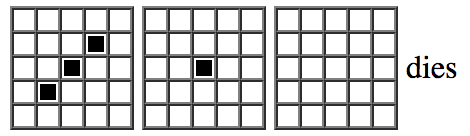
\includegraphics[scale=1]{img/1.png}
			\caption{Primer patrón}
			\label{fig:patron1}
		\end{center}
	\end{figure}

	Resultados obtenidos:
	\begin{figure}[H]
		\begin{center}
			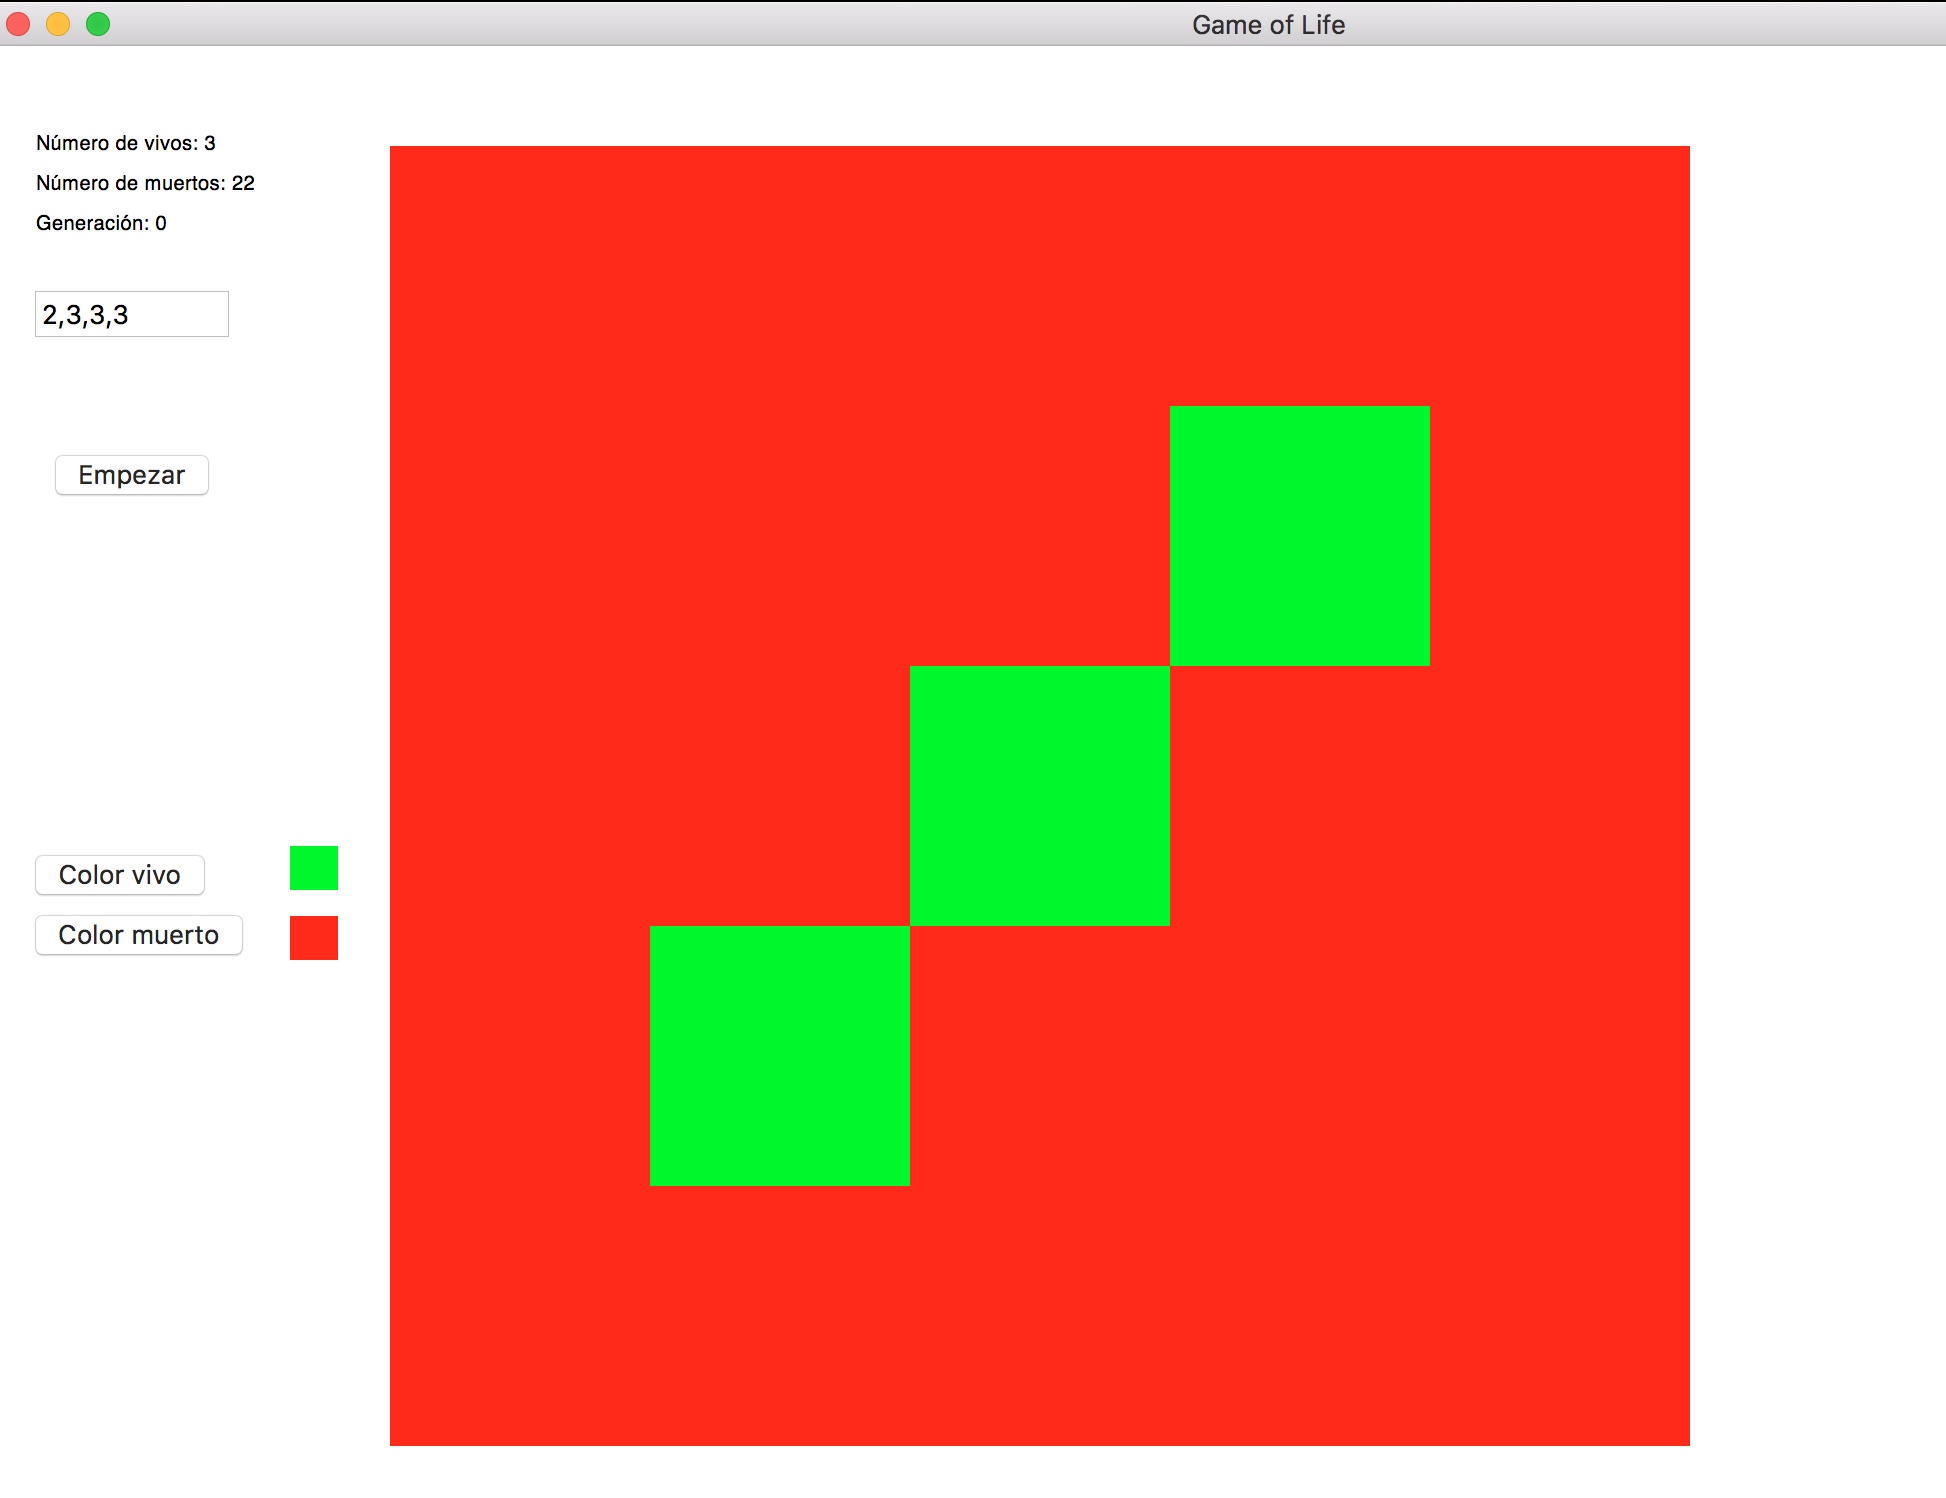
\includegraphics[scale=.4]{img/prueba1_1.png}
			\caption{Primer resultado obtenido(1)}
			\label{fig:prueba1_1}
		\end{center}
	\end{figure}
	\begin{figure}[H]
		\begin{center}
			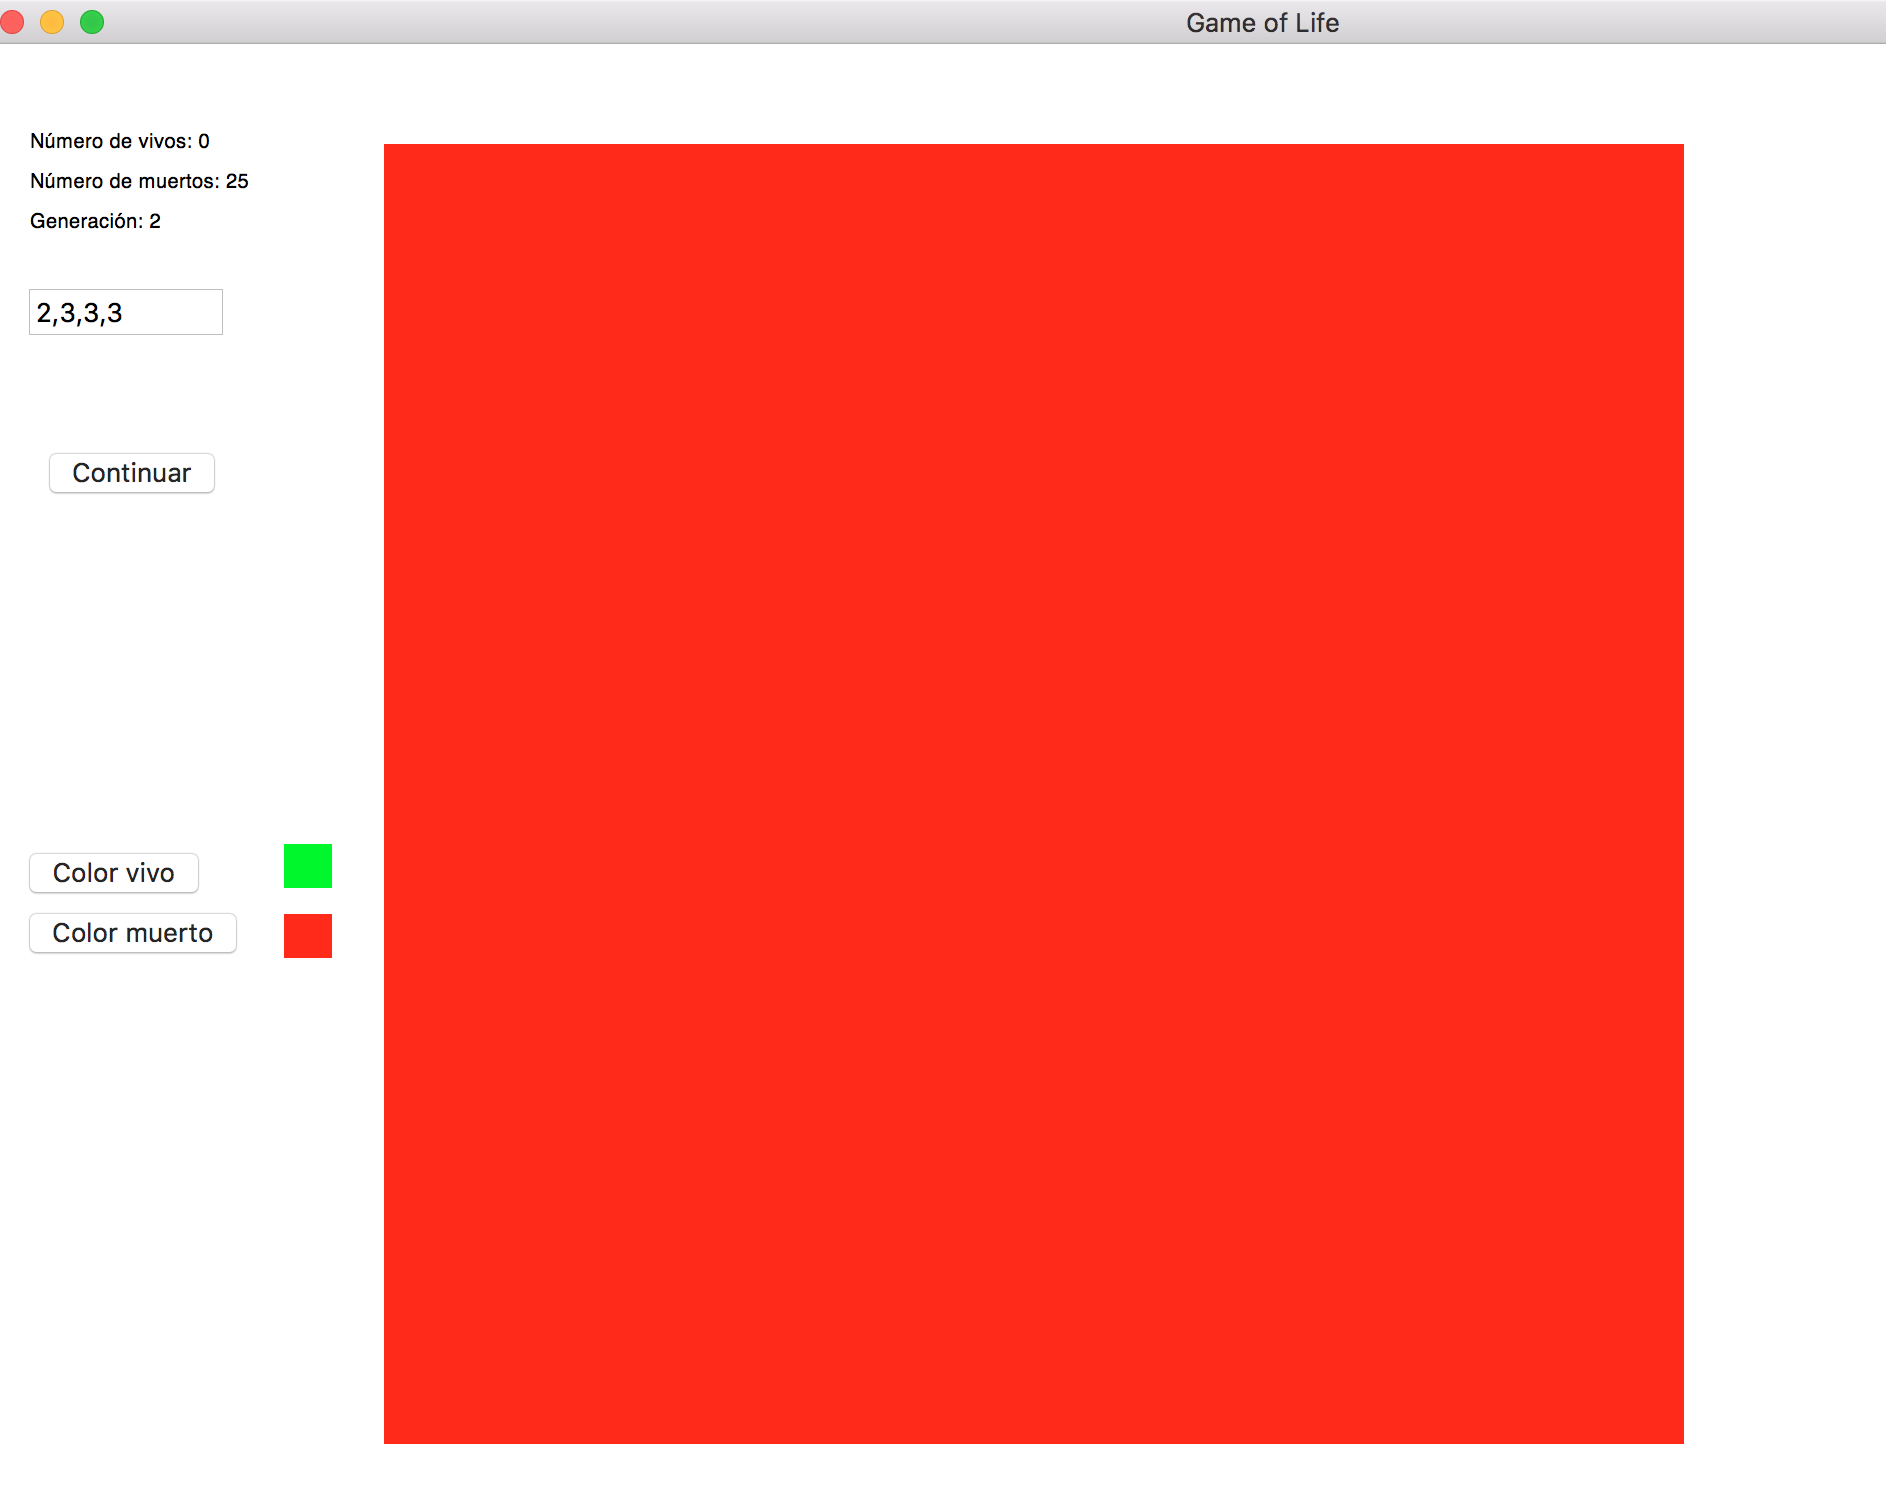
\includegraphics[scale=.4]{img/prueba1_2.png}
			\caption{Primer resultado obtenido(2)}
			\label{fig:prueba1_2}
		\end{center}
	\end{figure}

	Segundo patrón
	\begin{figure}[H]
		\begin{center}
			
\includegraphics[scale=1]{img/2.png}
			\caption{Segundo patrón}
			\label{fig:patron2}
		\end{center}
	\end{figure}

	Resultados obtenidos:
	\begin{figure}[H]
		\begin{center}
			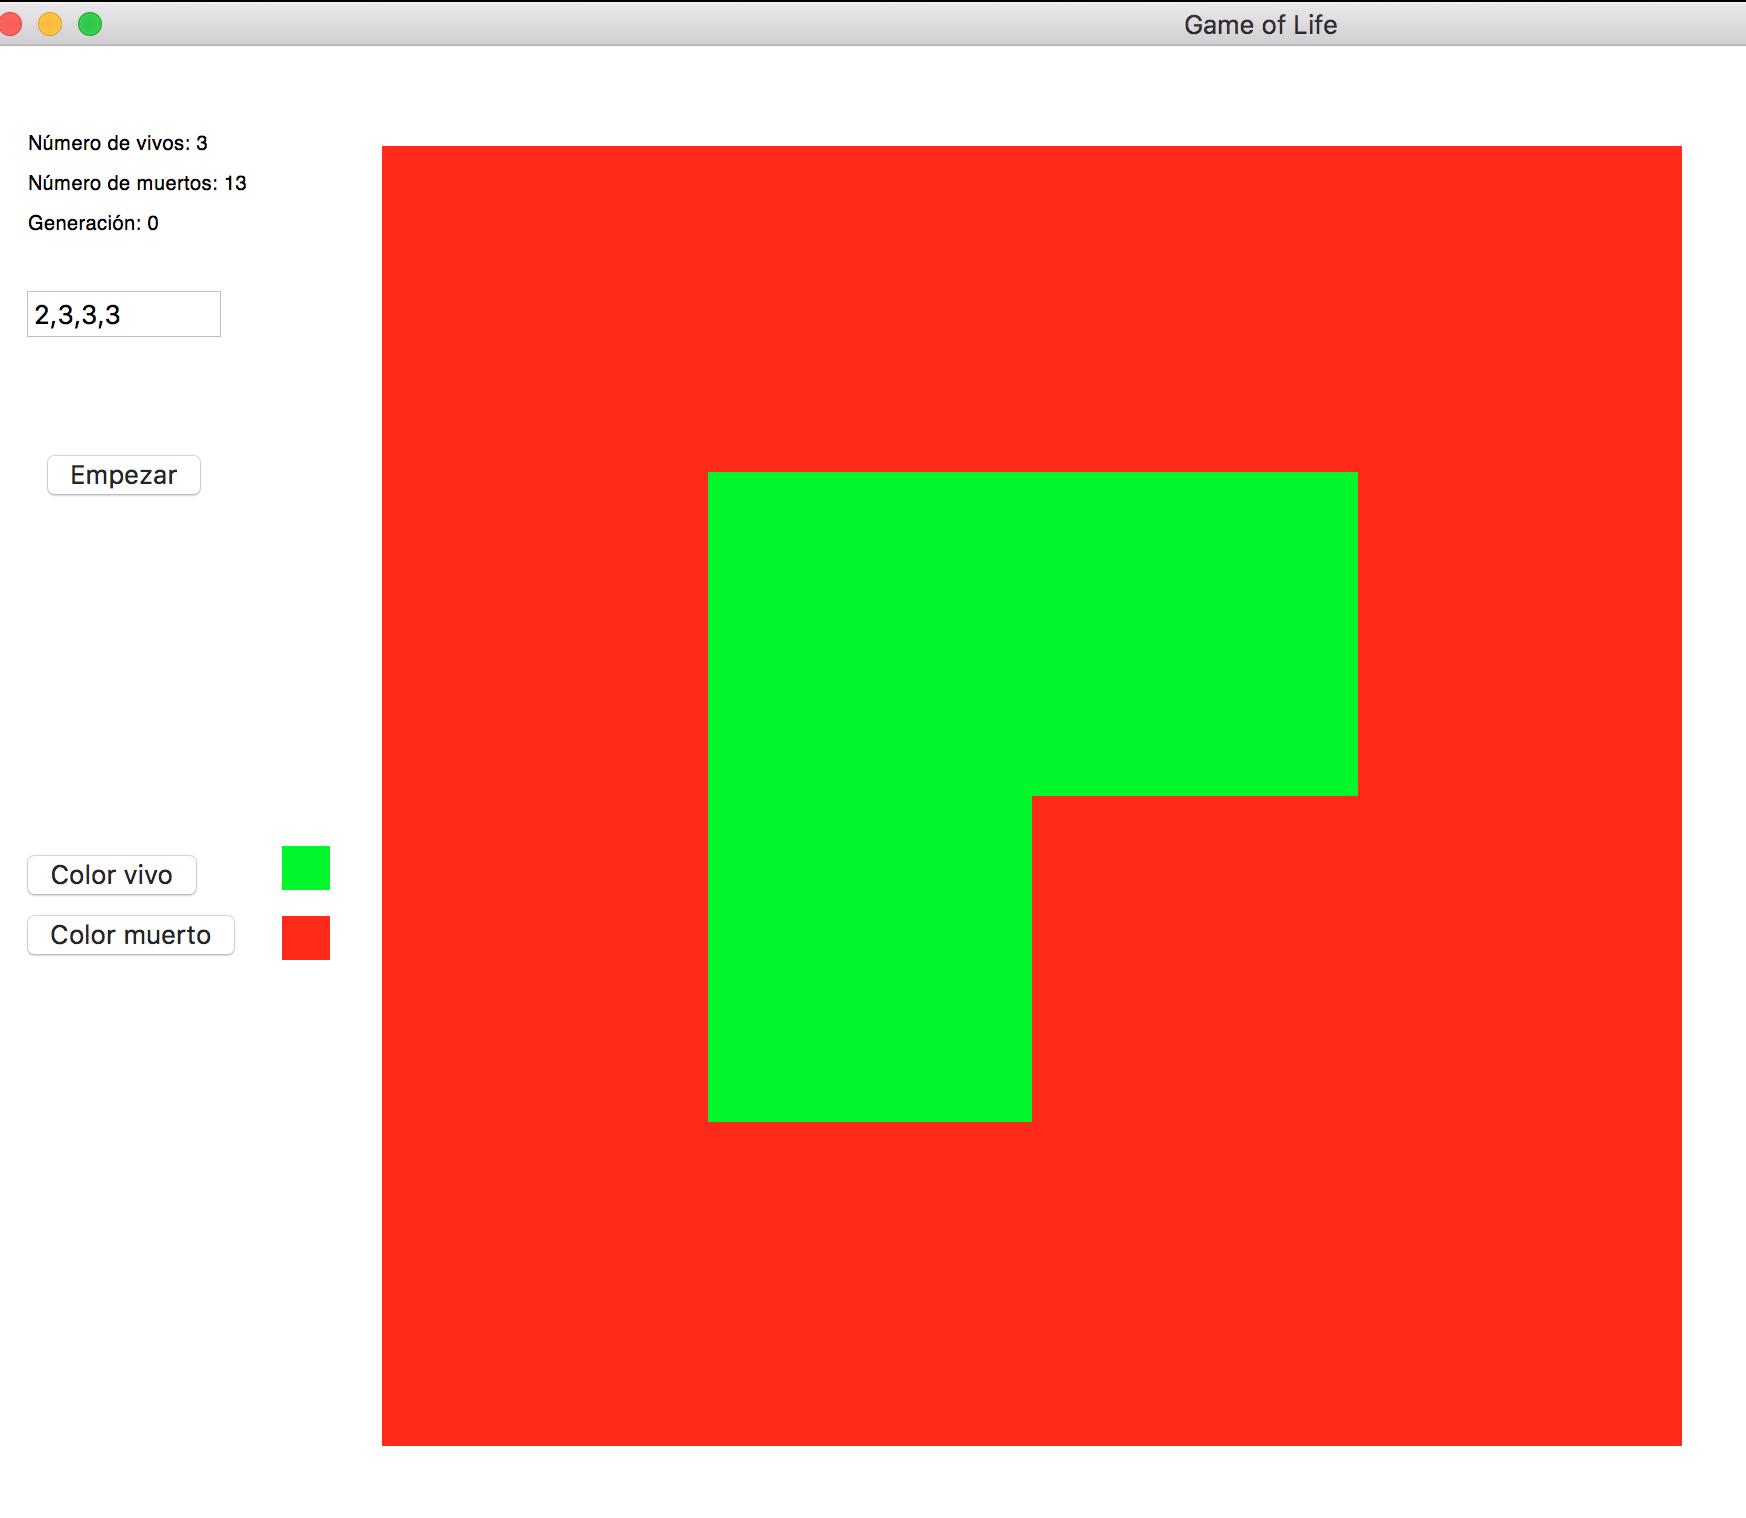
\includegraphics[scale=.4]{img/prueba2_1.png}
			\caption{Segundo resultado obtenido(1)}
			\label{fig:prueba2_1}
		\end{center}
	\end{figure}
	\begin{figure}[H]
		\begin{center}
			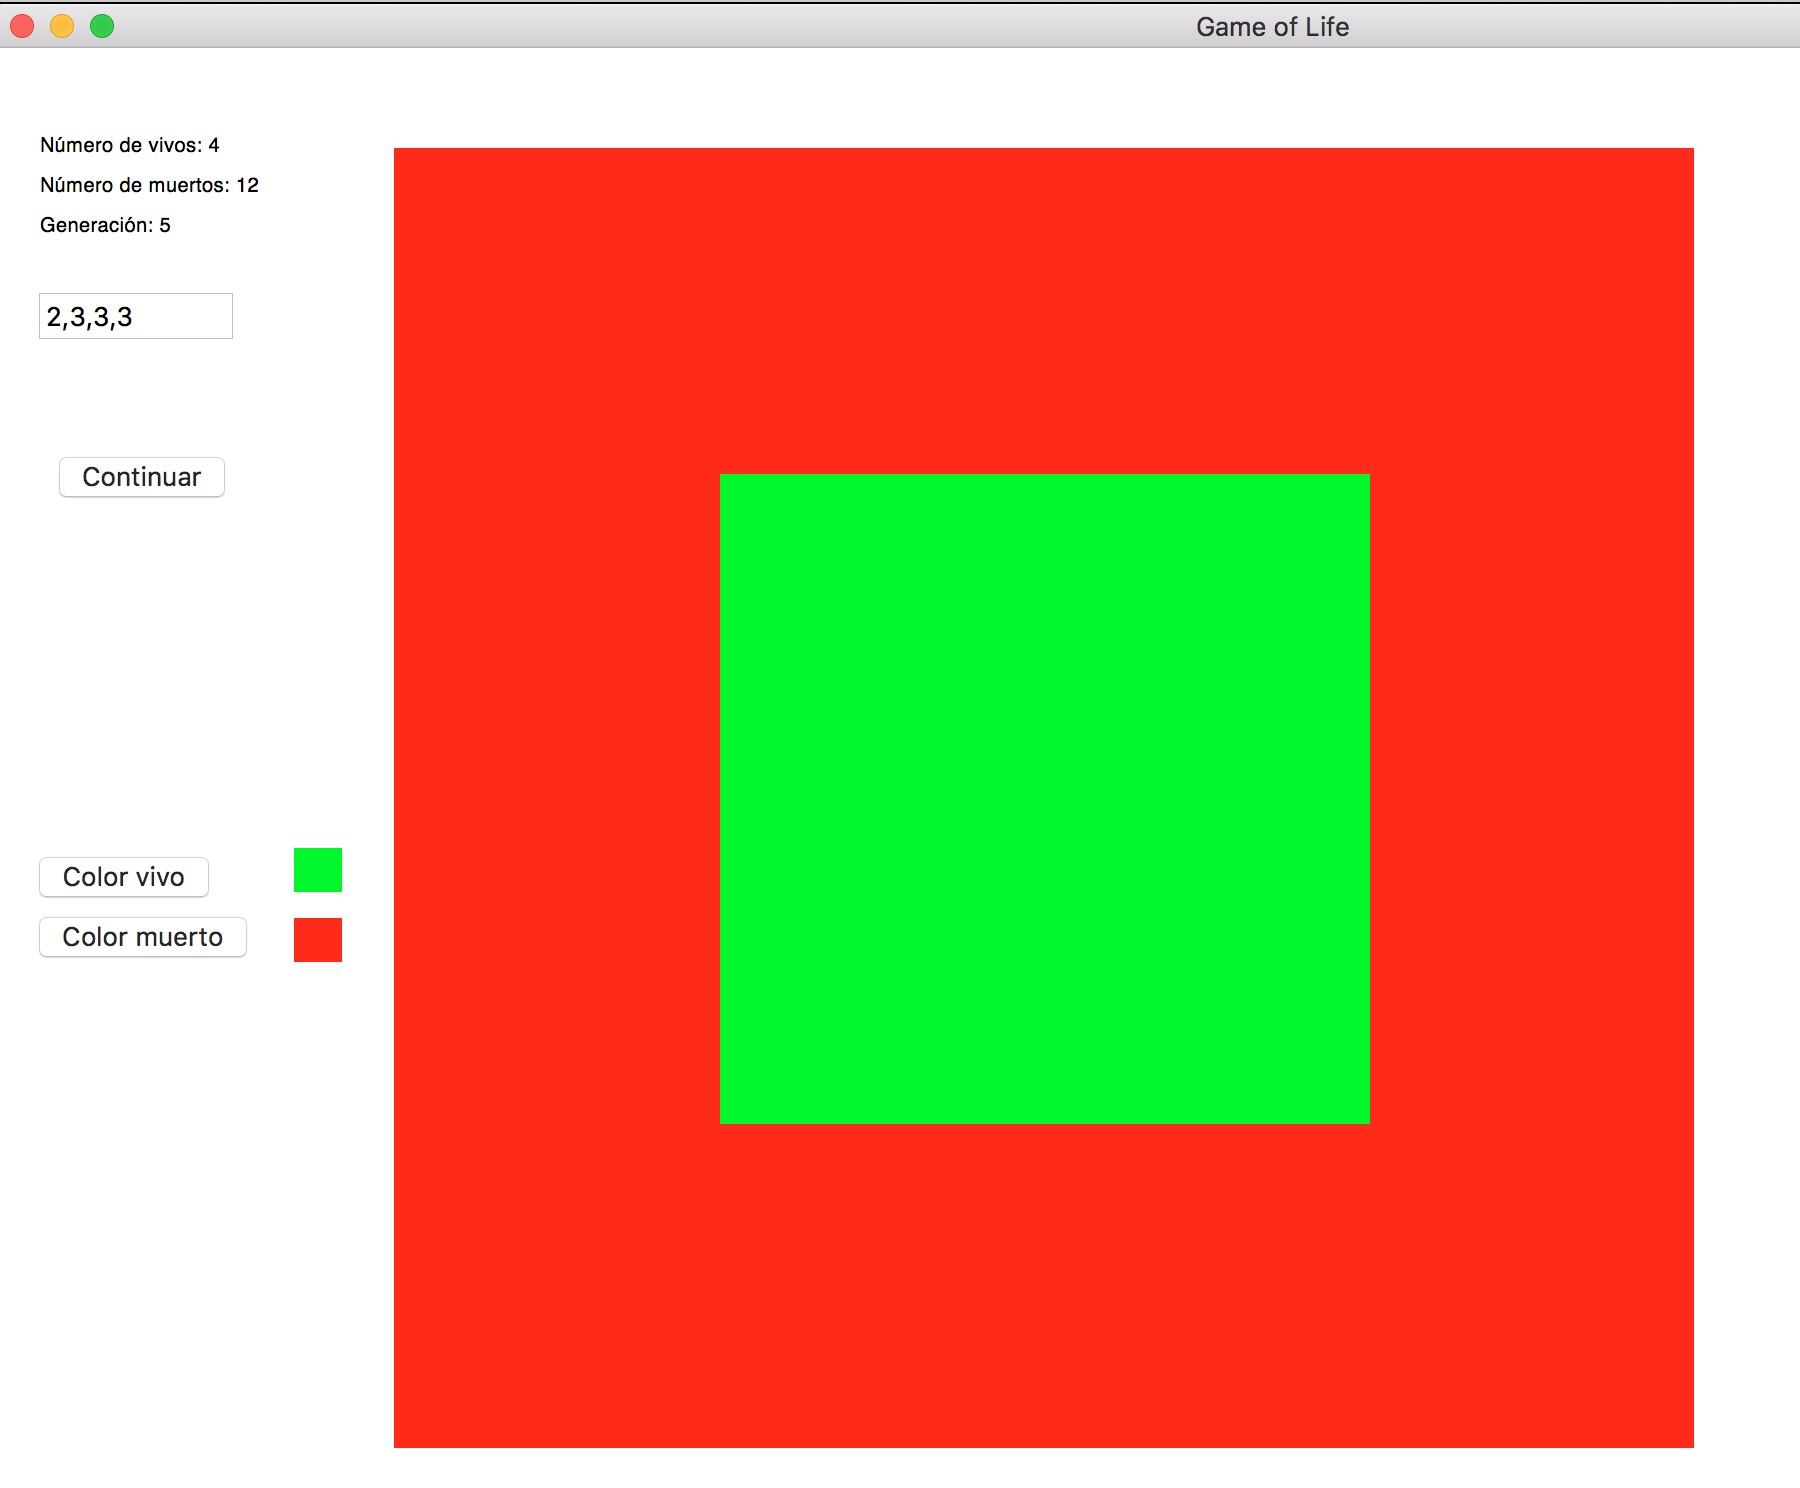
\includegraphics[scale=.4]{img/prueba2_2.png}
			\caption{Segundo resultado obtenido(2)}
			\label{fig:prueba2_2}
		\end{center}
	\end{figure}

	Tercer patrón
	\begin{figure}[H]
		\begin{center}
			
\includegraphics[scale=1]{img/3.png}
			\caption{Tercer patrón}
			\label{fig:patron3}
		\end{center}
	\end{figure}

	Resultados obtenidos:
	\begin{figure}[H]
		\begin{center}
			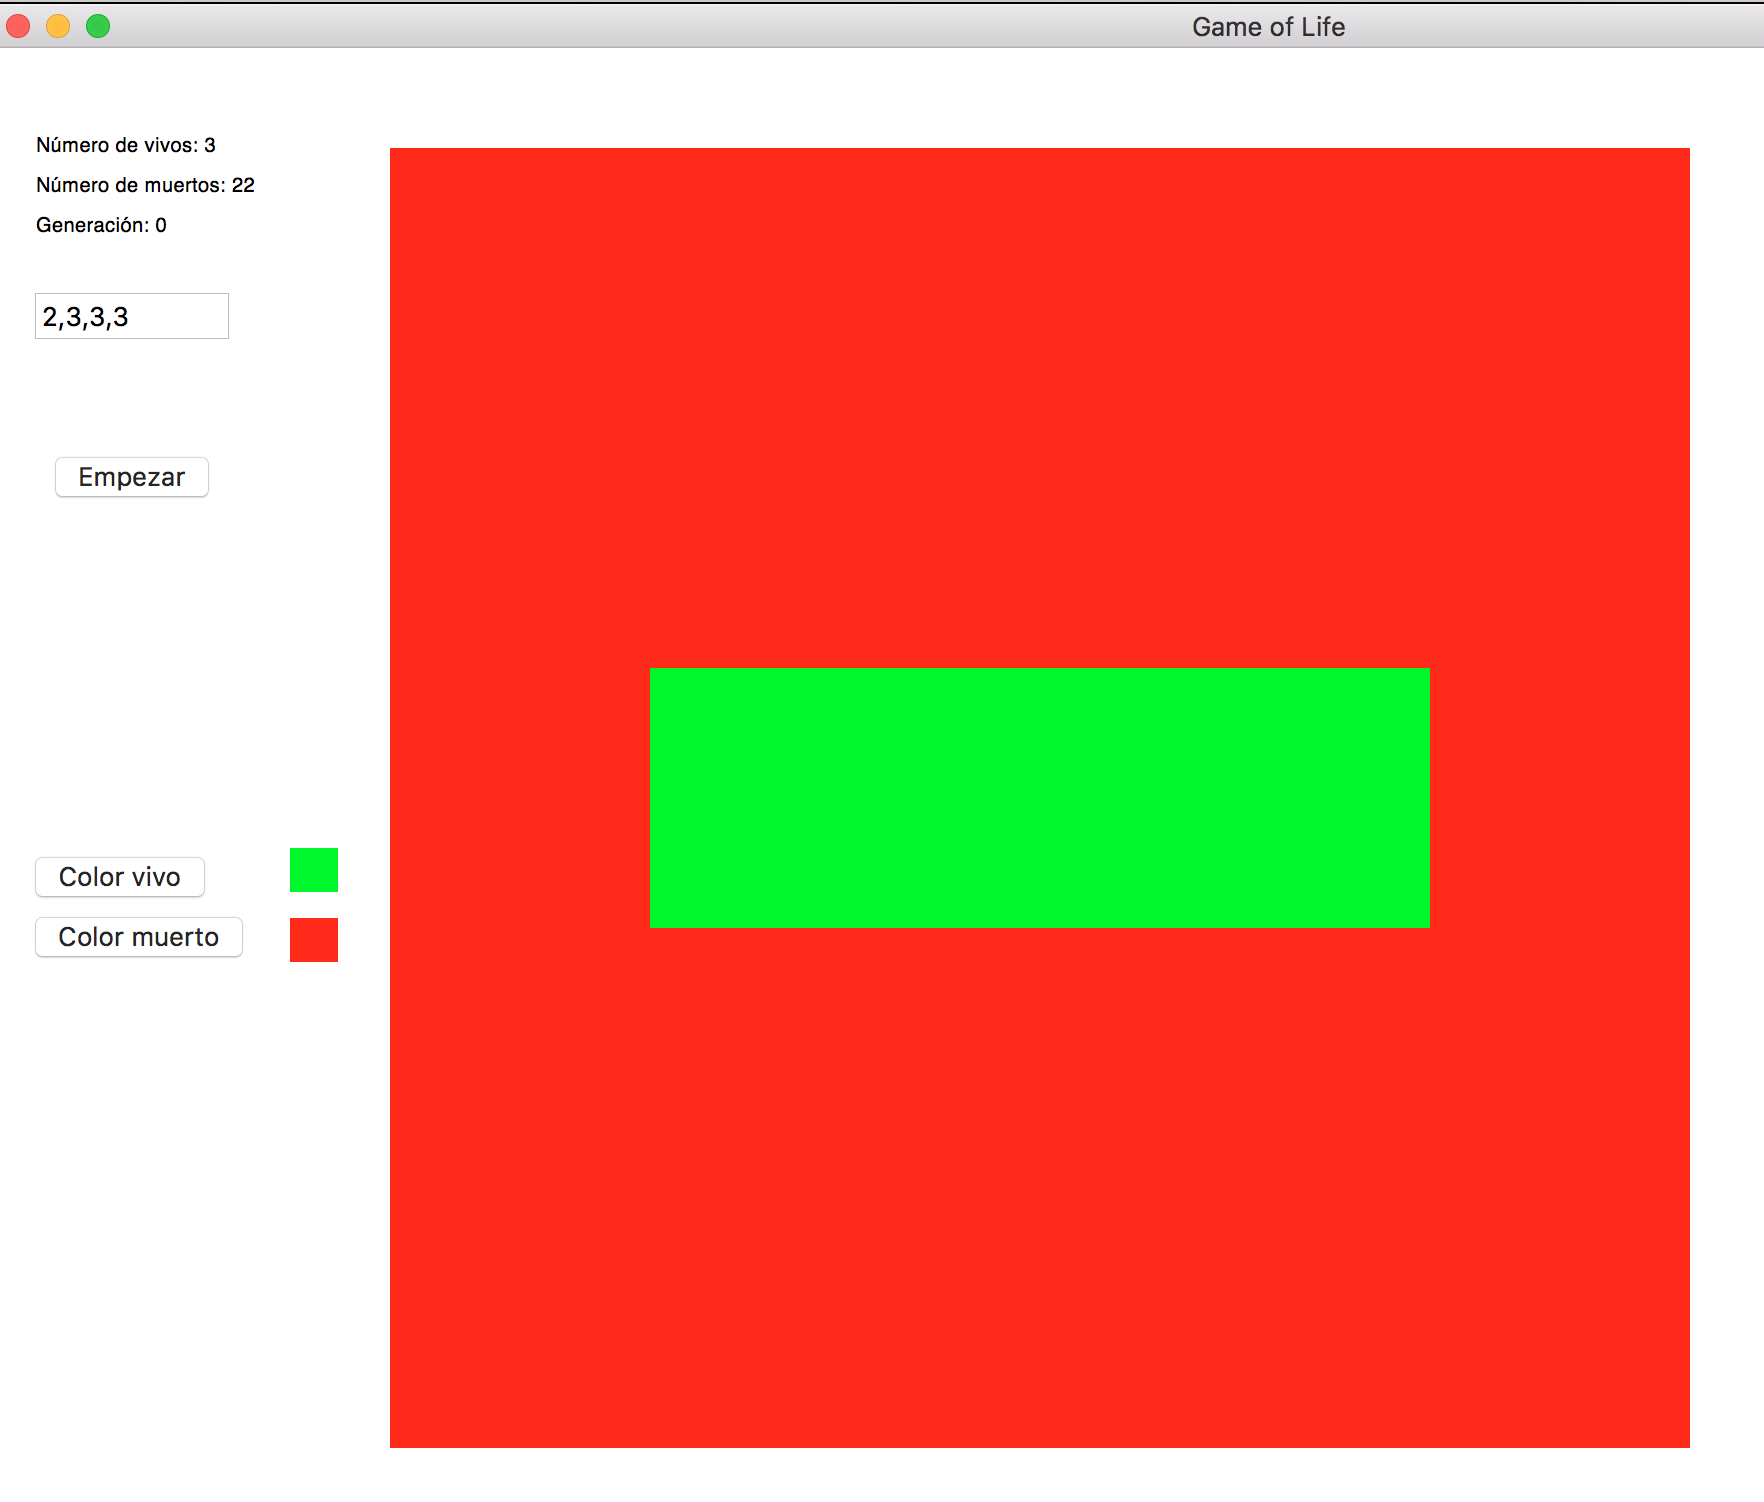
\includegraphics[scale=.4]{img/prueba3_1.png}
			\caption{Tercer resultado obtenido(1)}
			\label{fig:prueba3_1}
		\end{center}
	\end{figure}
	\begin{figure}[H]
		\begin{center}
			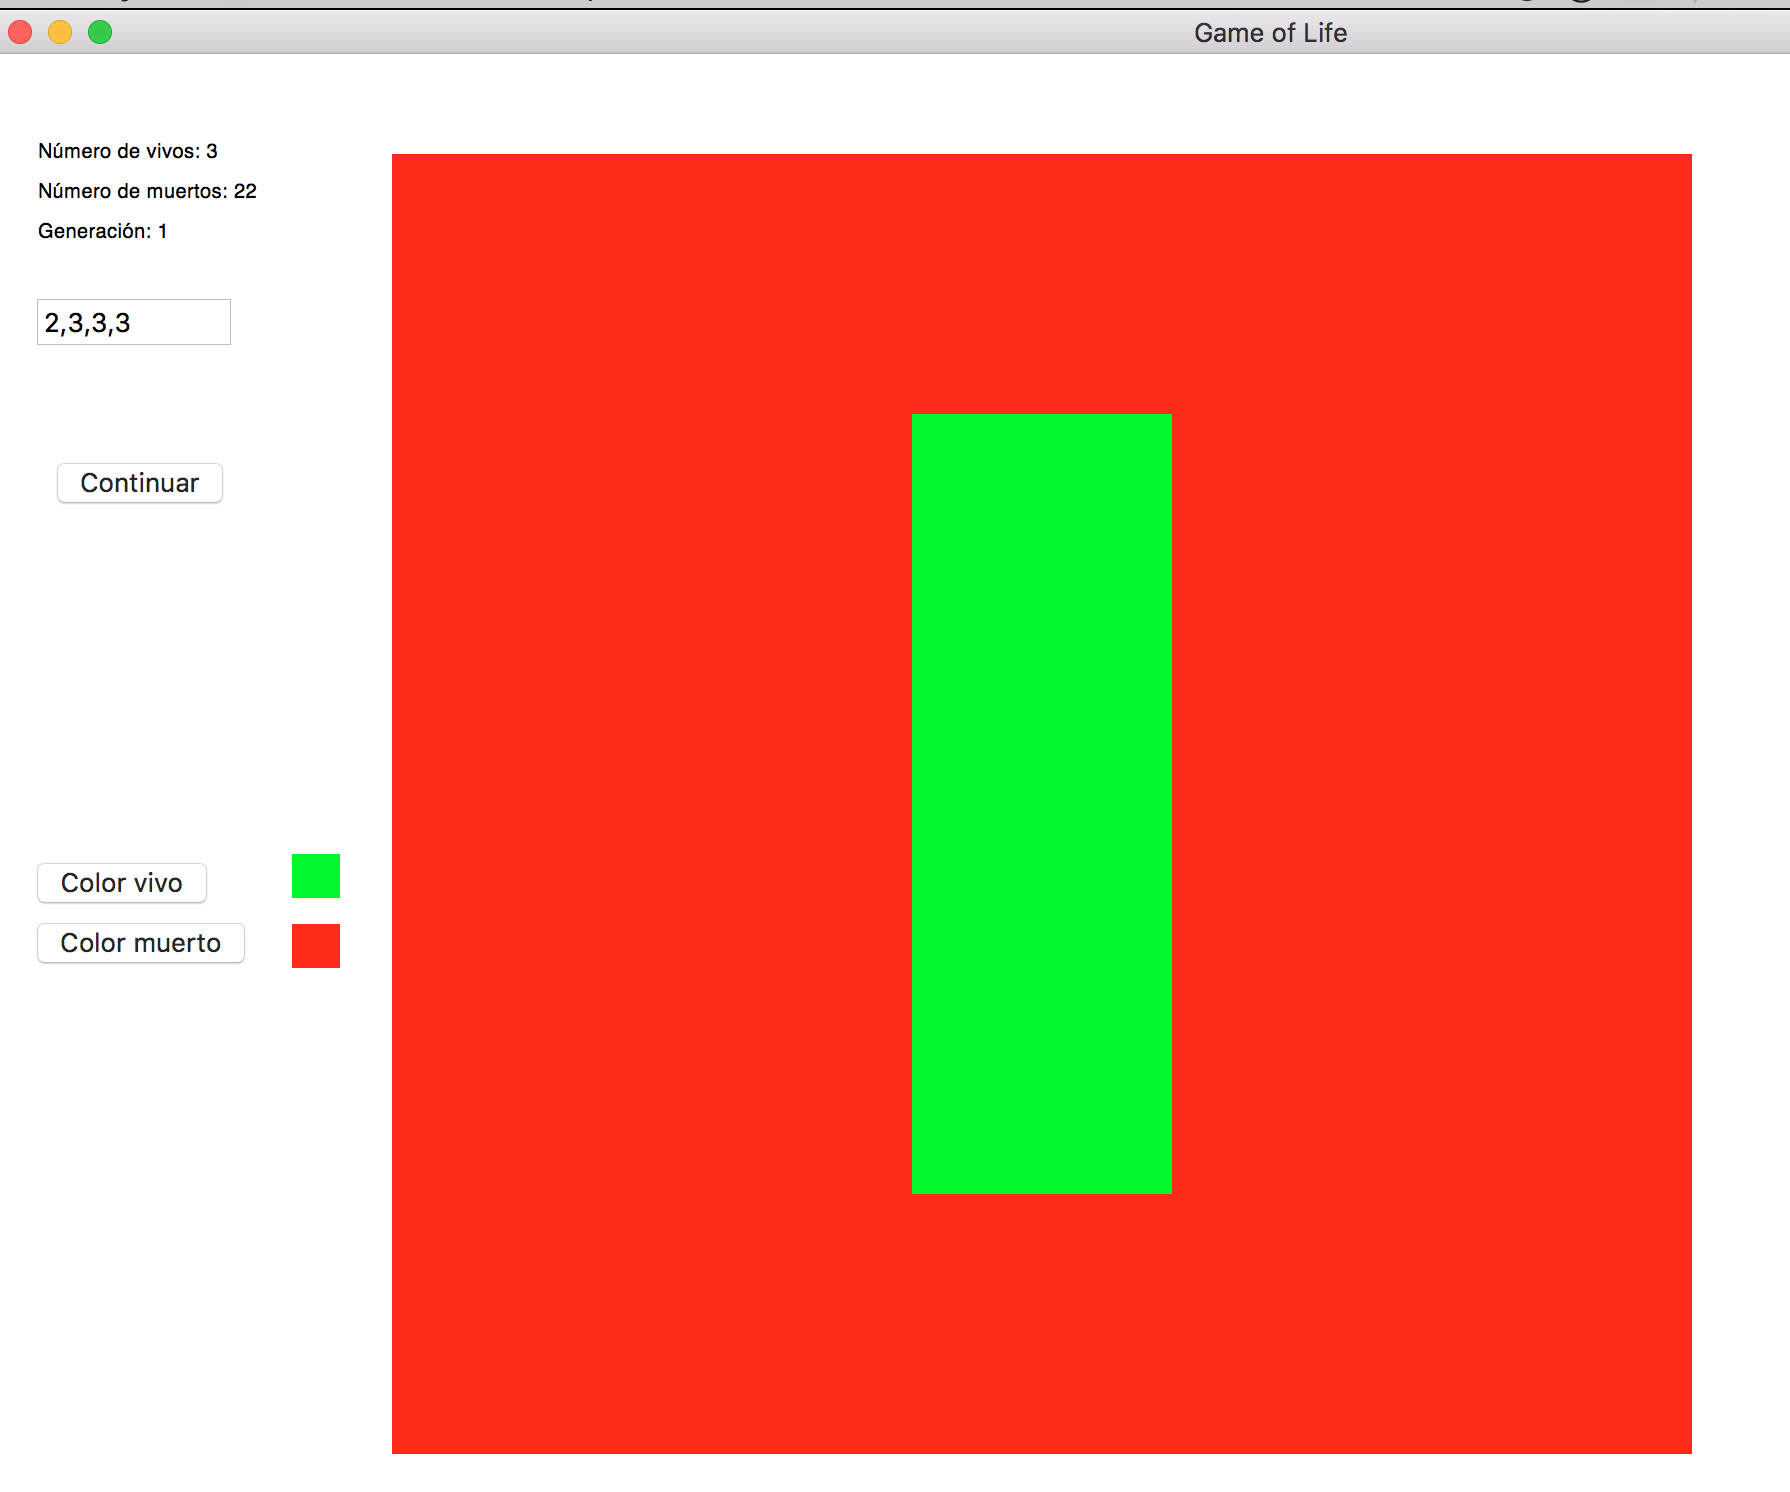
\includegraphics[scale=.4]{img/prueba3_2.png}
			\caption{Tercer resultado obtenido(2)}
			\label{fig:prueba3_2}
		\end{center}
	\end{figure}
	\begin{figure}[H]
		\begin{center}
			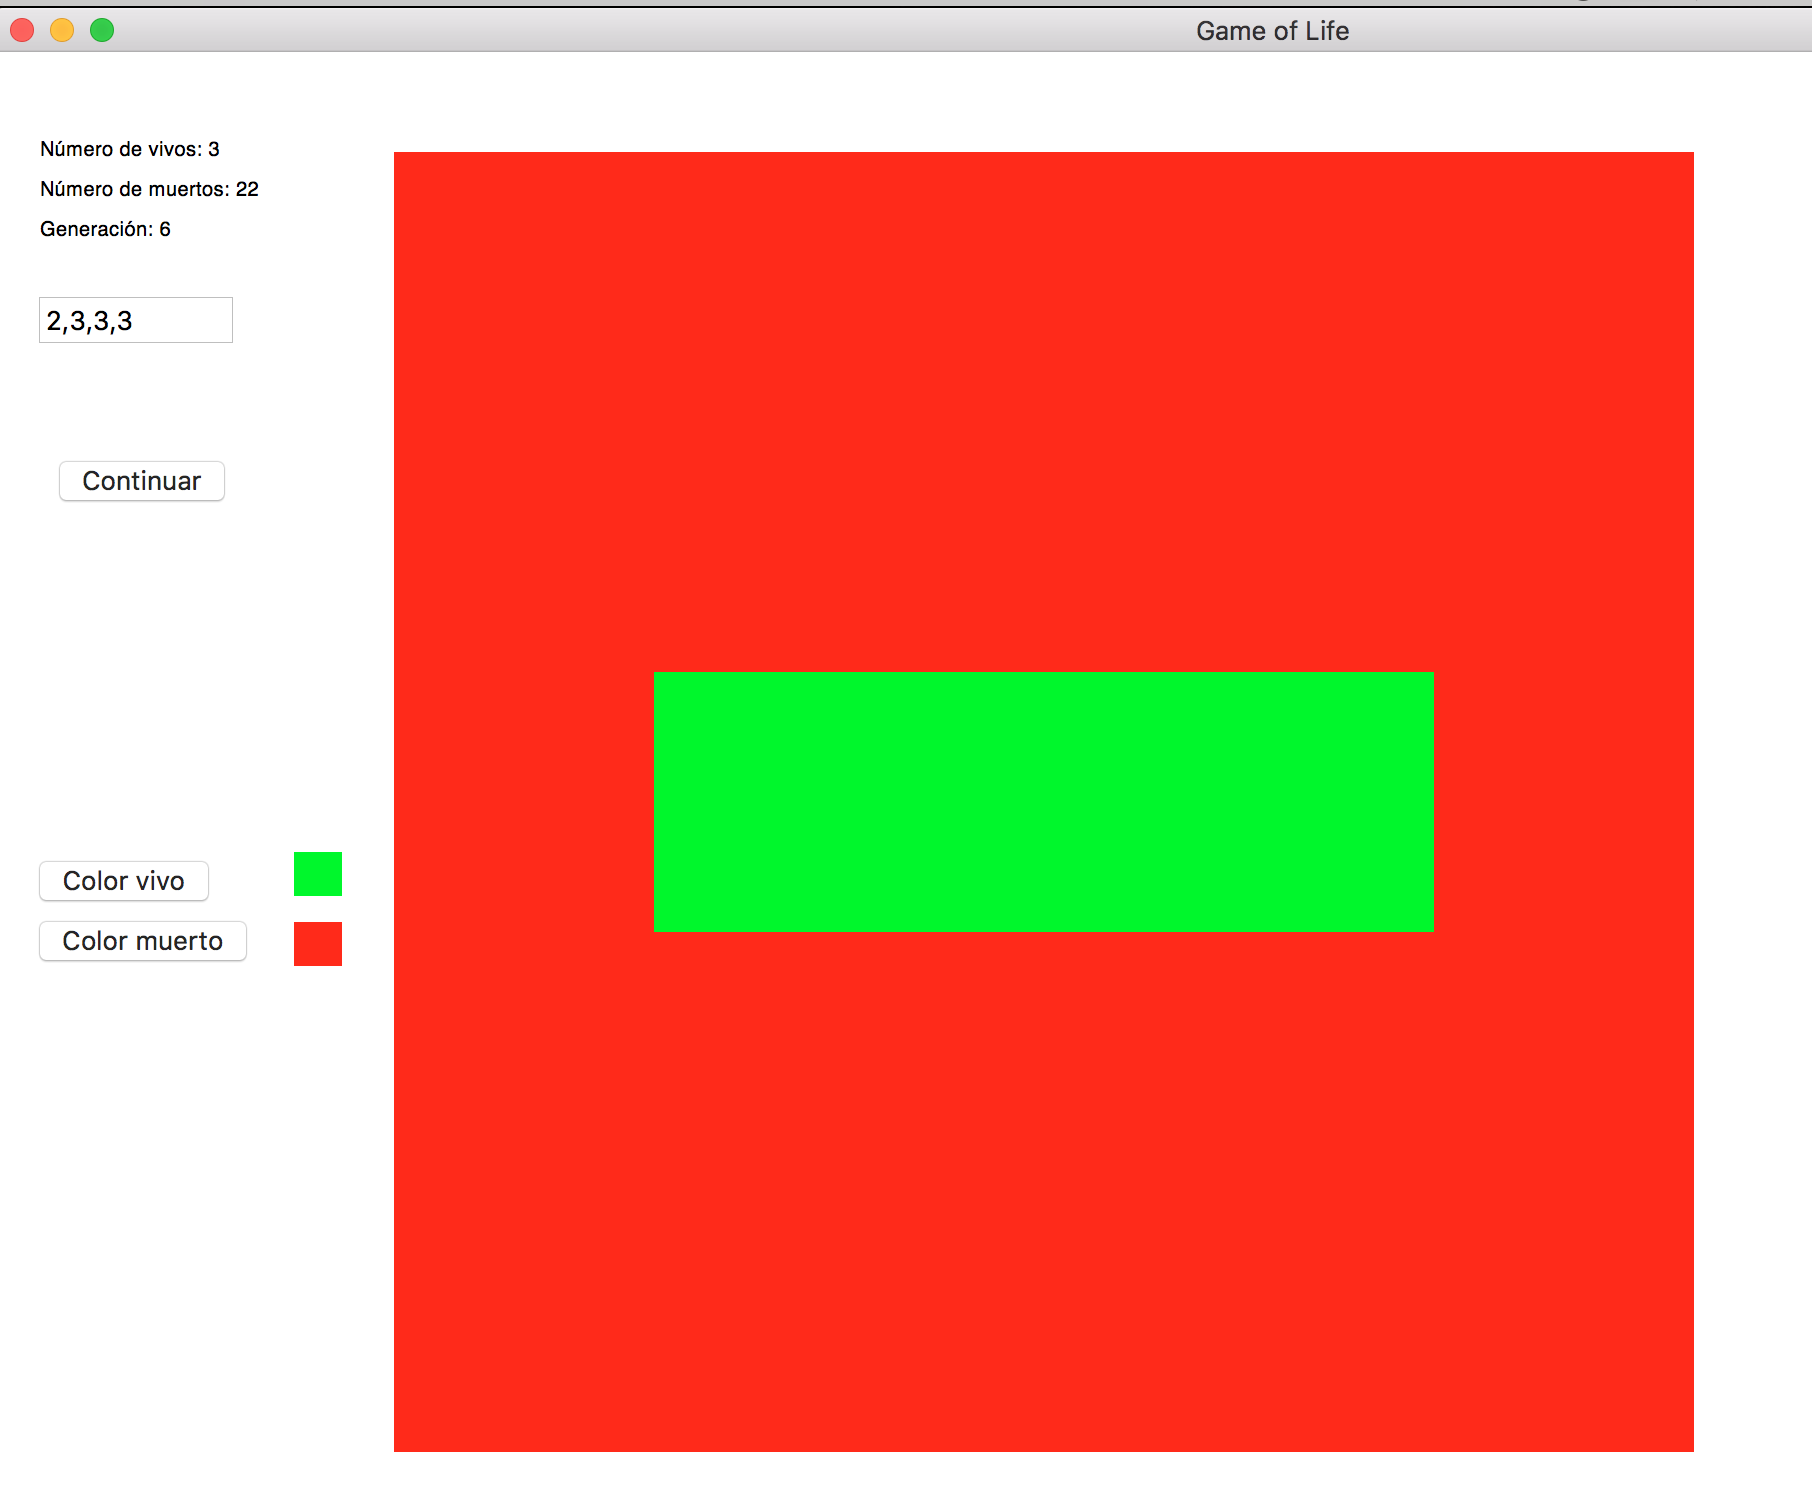
\includegraphics[scale=.4]{img/prueba3_3.png}
			\caption{Tercer resultado obtenido(3)}
			\label{fig:prueba3_3}
		\end{center}
	\end{figure}